\documentclass[aspectratio=169]{beamer}

\usetheme{default}
\usefonttheme{professionalfonts}
\setbeamertemplate{navigation symbols}{}
\setbeamertemplate{itemize items}[circle]
\setbeamercolor{itemize item}{fg=white}

\setbeamerfont{title}{series=\bfseries, size=\normalfont\Large}
\setbeamercolor{title}{fg=white}

\setbeamerfont{author}{size=\normalfont\small}
\setbeamercolor{author}{fg=white}

\setbeamerfont{frametitle}{series=\bfseries, size=\normalfont}
\setbeamercolor{frametitle}{fg=white}

\setbeamerfont{framesubtitle}{size=\normalfont\large}
\setbeamercolor{framesubtitle}{fg=white}

\setbeamercolor{background canvas}{bg=black}
\setbeamercolor{normal text}{fg=white}

\setbeamercolor{local structure}{fg=white}

\usepackage[utf8]{inputenc}
\usepackage[french]{babel}
\usepackage{amsmath}
\usepackage{amsfonts}
\usepackage{amssymb}
\usepackage{graphicx}
\usepackage[]{bm}
\usepackage[]{multimedia}
\usepackage[]{multicol}
\usepackage[squaren,Gray]{SIunits}

\graphicspath{{imgs/}}

\DeclareMathOperator*{\minimize}{minimiser~}
\DeclareMathOperator*{\maximize}{maximiser~}
\DeclareMathOperator*{\subjectto}{sous~la~contrainte~}


\usepackage{tikz} % Required for drawing custom shapes
\usetikzlibrary{arrows}
\usetikzlibrary{shapes.geometric, math, positioning, calc, patterns, angles, quotes}
\usetikzlibrary{patterns.meta,decorations.pathmorphing}




%\usepackage[]{listings}
\usepackage[many]{tcolorbox}
\tcbuselibrary{listings}

%% \definecolor{codegreen}{rgb}{0,0.8,0}
%% \definecolor{codegray}{rgb}{0.5,0.5,0.5}
%% %\definecolor{codepurple}{rgb}{0.58,0,0.82}
%% \definecolor{codepurple}{rgb}{0,0.8,0}
%% \definecolor{backcolour}{rgb}{0.0, 0.0, 0.0}

\definecolor{codegreen}{rgb}{0,0.6,0}
\definecolor{codered}{rgb}{0.6,0.1,0}
\definecolor{codegray}{rgb}{0.5,0.5,0.5}
\definecolor{codepurple}{rgb}{0.58,0,0.82}
\definecolor{backcolour}{rgb}{0, 0, 0}
\definecolor{lightgray}{gray}{0.95}
\definecolor{codeblue}{rgb}{0.117,0.403,0.713}

\newcounter{ipythcntr}
\renewcommand{\theipythcntr}{\texttt{[\arabic{ipythcntr}]}}
\newcommand{\ipin}[1][]{
  \stepcounter{ipythcntr}
  \hspace{-10pt}
  \color{codeblue}In  \theipythcntr}
\newcommand{\ipout}[1][\theipythcntr]{
  \hspace{-10pt}
  \color{codered}Out \theipythcntr}

\lstdefinestyle{mystyle}{
  language=Python,
  moredelim=[is][\ipin]{In[}{]},
  moredelim=[is][\ipout]{Out[}{]},
  backgroundcolor=\color{backcolour},
  commentstyle=\color{codegreen},
  keywordstyle=\color{magenta},
  numberstyle=\tiny\color{codegray},
  stringstyle=\color{codepurple},
  basicstyle=\ttfamily\footnotesize,
  breakatwhitespace=false,
  breaklines=true,
  captionpos=b,
  keepspaces=true,
  numbers=left,
  numbersep=5pt,
  showspaces=false,
  showstringspaces=false,
  showtabs=false,
  tabsize=2,
}

\lstset{style=mystyle}


\title{Introduction à Python}
\author{Jean-Christophe LOISEAU}
\institute{Arts \& Métiers Institute of Technology, 2021-2022}
\date{}

\begin{document}





\frame{\titlepage}





\begin{frame}
  \begin{minipage}{.64\textwidth}
    \textbf{\alert{NumPy}} : bibliothèque (ou package) pour \textbf{Python} destinée à manipuler des \textbf{matrices} ou \textbf{tableaux multidimensionels} ainsi que des fonctions mathématiques opérant sur ces tableaux.
  \end{minipage}%
  \hfill
  \begin{minipage}{.32\textwidth}
    \centering
    
\includegraphics[width=\textwidth]{numpy_logo}
  \end{minipage}

  \vspace{-1cm}
\end{frame}





%% {
%%   \setbeamercolor{background canvas}{bg=white}
%%   \frame{
%%     \vfill
%%     \centering
%%     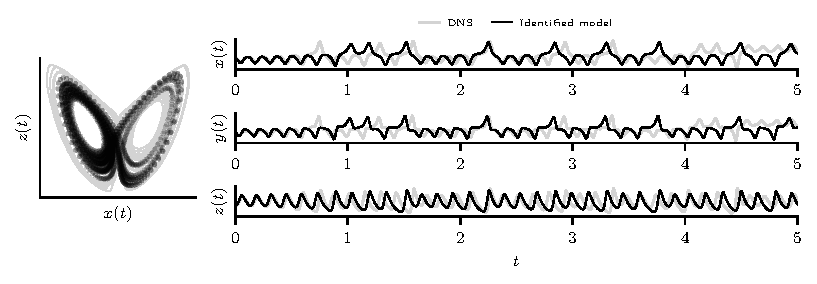
\includegraphics[width=\textwidth]{attractor_comparison_bis}
%%     \vfill
%%   }
%% }

\begin{frame}
  \vfill
  \centering
  \centering

  Comment calculer $\bm{x} \cdot \bm{y}$ avec $\bm{x}, \bm{y} \in \mathbb{R}^n$ ?

  \vfill
\end{frame}

\frame{
  \vfill
  \[
  \bm{x} \cdot \bm{y} = \sum_{i=1}^n x_i y_i
  \]
  \vfill
}


\begin{frame}[fragile]{}{}
  \vfill
  \begin{lstlisting}%[language=Python]

    def produit_scalaire(x, y):

        # Initialise la variable.
        z = 0

        # Calcul le produit scalaire.
        for i in range(len(x)):
            z = z + x[i] * y[i]

        return z

  \end{lstlisting}
  \vfill
\end{frame}




{
  \setbeamercolor{background canvas}{bg=white}
  \begin{frame}[fragile]{}{}
    \vfill
    \begin{lstlisting}[backgroundcolor=\color{white}, basicstyle=\ttfamily\footnotesize\color{black}]
      In[:] x, y = npr.rand(100_000), npr.rand(100_000)
    
      In[:] %%timeit
              produit_scalaire(x, y)
    \end{lstlisting}
    \hspace{1cm}
    \footnotesize{\texttt{\color{black}{
          \unit{26.9}{\milli\second} $\pm$ \unit{110}{\micro\second} (mean $\pm$ std. dev. of 7 runs, 100 loops each)
    }}}
    
    \vfill
  \end{frame}
}


\begin{frame}[fragile]{}{}
  \vfill
  \begin{lstlisting}%[language=Python]

    def produit_scalaire(x, y):
        # Calcul le produit scalaire.
        return np.sum(x * y)
  \end{lstlisting}
  \vfill
\end{frame}




{
  \setbeamercolor{background canvas}{bg=white}
  \begin{frame}[fragile]{}{}
    \vfill
    \begin{lstlisting}[backgroundcolor=\color{white}, basicstyle=\ttfamily\footnotesize\color{black}]
      In[:] x, y = npr.rand(100_000), npr.rand(100_000)
      
      In[:] %%timeit
              produit_scalaire(x, y)
    \end{lstlisting}
    \hspace{1cm}
    \footnotesize{\texttt{\color{black}{
          \unit{100}{\micro\second} $\pm$ \unit{1.85}{\micro\second} (mean $\pm$ std. dev. of 7 runs, 10000 loops each)
    }}}
    
    \vfill
  \end{frame}
}





{
  \setbeamercolor{background canvas}{bg=white}
  \begin{frame}[fragile]{}{}
    \vfill
    \begin{lstlisting}[backgroundcolor=\color{white}, basicstyle=\ttfamily\footnotesize\color{black}]
      In[:] x, y = npr.rand(100_000), npr.rand(100_000)
      
      In[:] %%timeit
              np.vdot(x, y)    # Produit scalaire en NumPy.
    \end{lstlisting}
    \hspace{1cm}
    \footnotesize{\texttt{\color{black}{
          \unit{25}{\micro\second} $\pm$ \unit{8.95}{\micro\second} (mean $\pm$ std. dev. of 7 runs, 10000 loops each)
    }}}
    
    \vfill
  \end{frame}
}



\frame{
  \vfill
  \centering

  Comment calculer $\| \bm{A} - \bm{B} \|_2$ avec $\bm{A}, \bm{B} \in \mathbb{R}^{m \times n}$ ?

  \vfill
}

\frame{
  \vfill
  \centering

  \[
  \| \bm{A} - \bm{B} \|_2 = \sqrt{\sum_{i=1}^m \sum_{j=1}^n (A_{ij} - B_{ij})^2}
  \]

  \vfill
}

\begin{frame}[fragile]{}{}
  \vfill
  \begin{lstlisting}
    def distance(A, B):
        # Taille des tableaux.
        m, n = A.shape

        # Initialise la variable.
        d = 0

        # Calcul la distance
        for i in range(m):
            for j in range(n):
                d += (A[i, j] - B[i, j])**2

        return np.sqrt(d)
  \end{lstlisting}
  \vfill
\end{frame}

{
  \setbeamercolor{background canvas}{bg=white}
  \begin{frame}[fragile]{}{}
    \vfill
    \begin{lstlisting}[backgroundcolor=\color{white}, basicstyle=\ttfamily\footnotesize\color{black}]
      In[:] A, B = npr.rand(1000, 1000), npr.rand(1000, 1000)
      
      In[:] %%timeit
              distance(A, B)
    \end{lstlisting}
    \hspace{1cm}
    \footnotesize{\texttt{\color{black}{
          \unit{615}{\milli\second} $\pm$ \unit{22.3}{\milli\second} (mean $\pm$ std. dev. of 7 runs, 1 loop each)
    }}}
    
    \vfill
  \end{frame}
}





\begin{frame}[fragile]{}{}
  \vfill
  \begin{lstlisting}
    def distance(A, B):
        d = np.sum( (A-B)**2 )
        return np.sqrt(d)
  \end{lstlisting}
  \vfill
\end{frame}

{
  \setbeamercolor{background canvas}{bg=white}
  \begin{frame}[fragile]{}{}
    \vfill
    \begin{lstlisting}[backgroundcolor=\color{white}, basicstyle=\ttfamily\footnotesize\color{black}]
      In[:] A, B = npr.rand(1000, 1000), npr.rand(1000, 1000)
      
      In[:] %%timeit
              distance(A, B)
    \end{lstlisting}
    \hspace{1cm}
    \footnotesize{\texttt{\color{black}{
          \unit{4.23}{\milli\second} $\pm$ \unit{69.3}{\micro\second} (mean $\pm$ std. dev. of 7 runs, 100 loops each)
    }}}
    
    \vfill
  \end{frame}
}

{
  \setbeamercolor{background canvas}{bg=white}
  \begin{frame}[fragile]{}{}
    \vfill
    \begin{lstlisting}[backgroundcolor=\color{white}, basicstyle=\ttfamily\footnotesize\color{black}]
      In[:] A, B = npr.rand(1000, 1000), npr.rand(1000, 1000)
      
      In[:] %%timeit
              npl.norm(A-B)     # Definition de la norme en NumPy.
    \end{lstlisting}
    \hspace{1cm}
    \footnotesize{\texttt{\color{black}{
          \unit{2.98}{\milli\second} $\pm$ \unit{77.1}{\micro\second} (mean $\pm$ std. dev. of 7 runs, 100 loops each)
    }}}
    
    \vfill
  \end{frame}
}




\frame{
  \vfill
  \centering
  \textbf{La méthode des moindres-carrés}
  \vfill
}

{
  \setbeamercolor{background canvas}{bg=white}
  \begin{frame}[fragile]{}{}
    \vfill
    \centering
    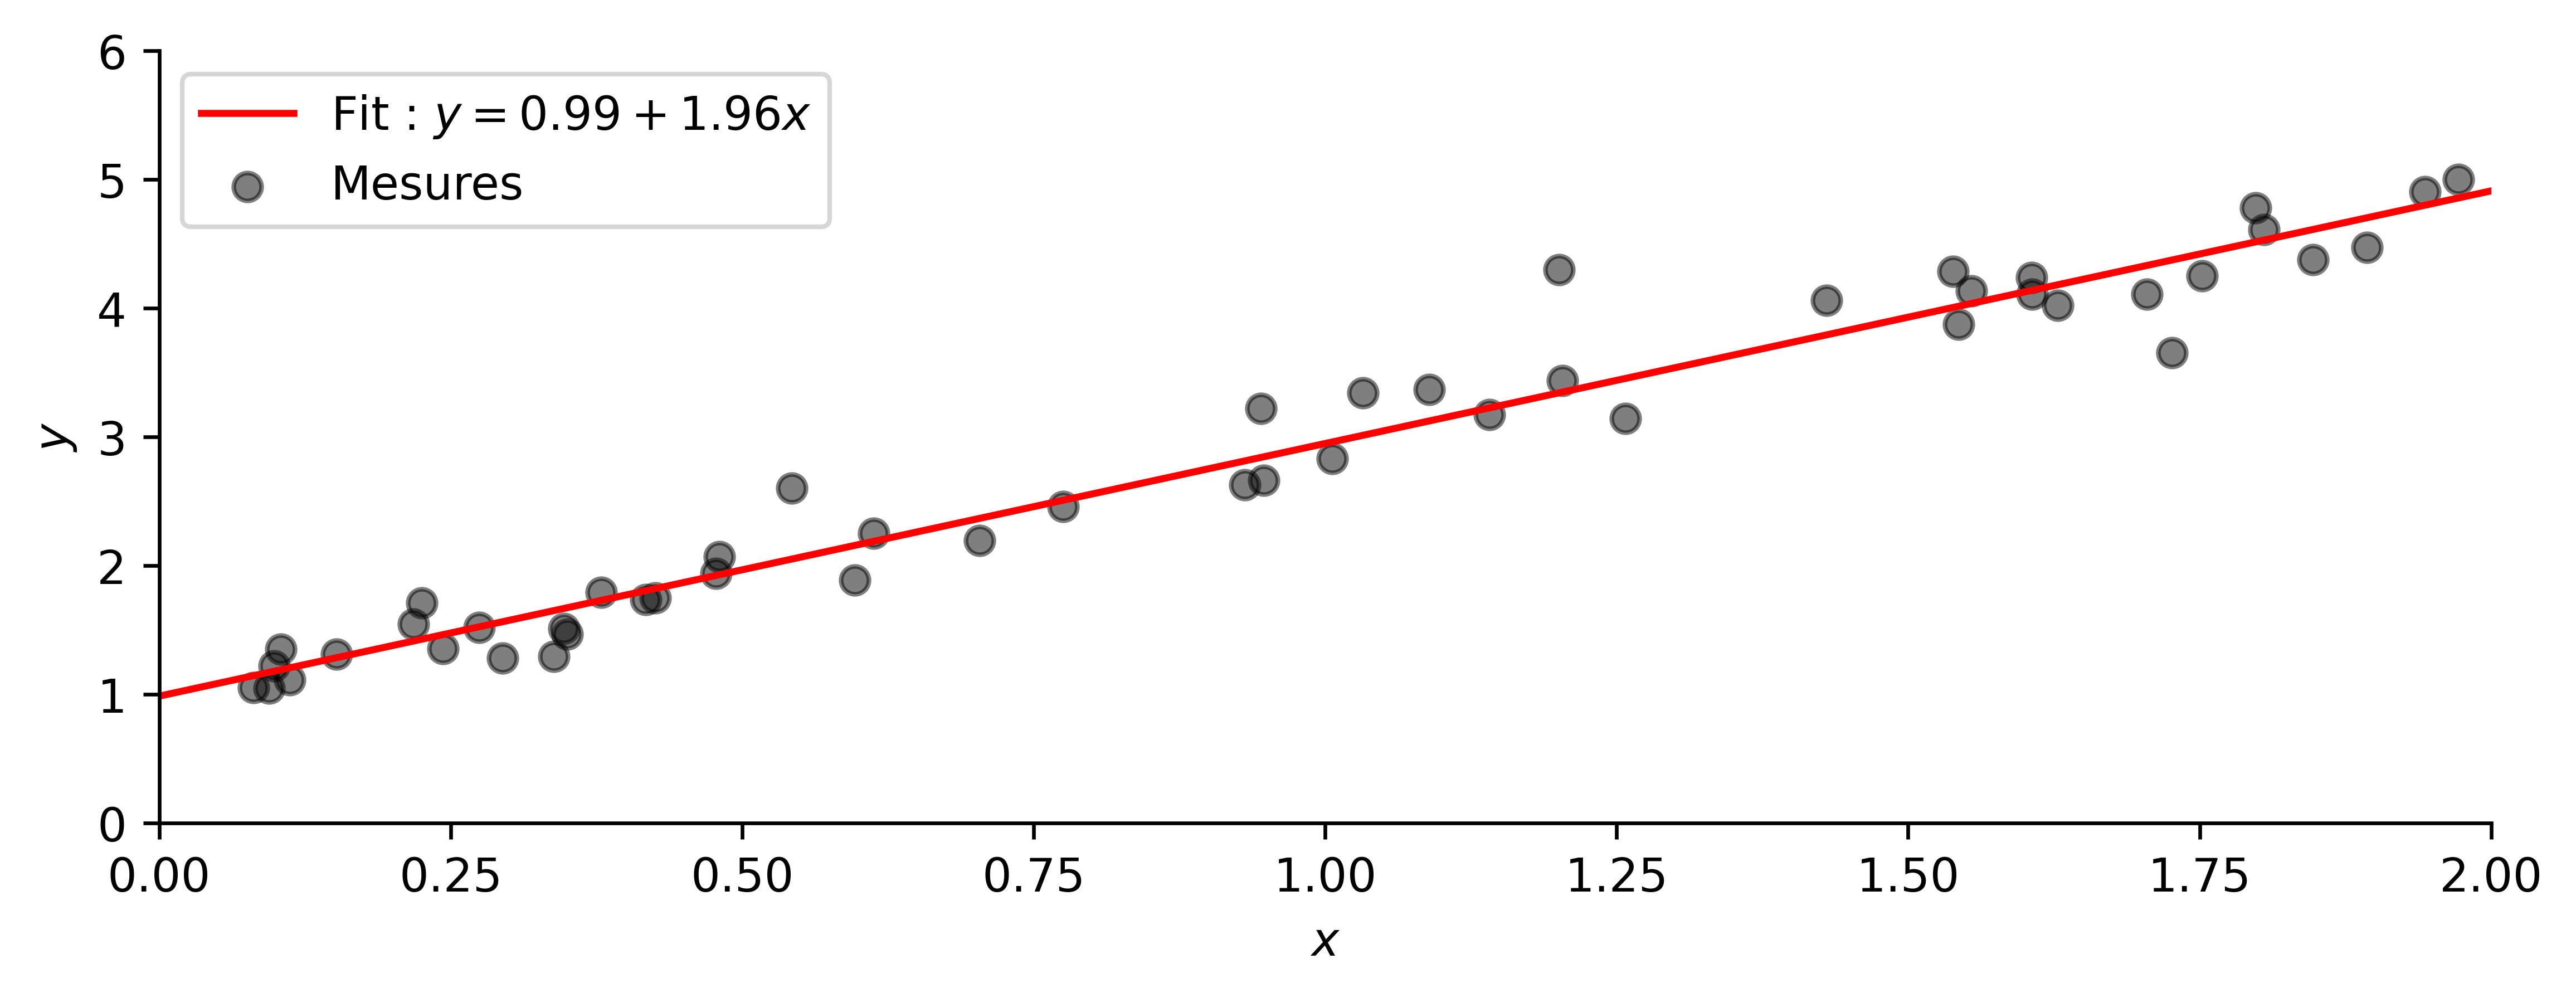
\includegraphics[width=\textwidth]{least_squares_ex}
    \vfill
  \end{frame}
}

\begin{frame}
  \vfill
  \centering

  Comment trouver l'équation de la droite $\hat{y} = ax + b$ \\
  qui approxime au mieux les données $(\bm{x}, \bm{y})$ ?

  \vfill
\end{frame}

\begin{frame}
  \vfill
  \textbf{Mesure de l'erreur :} Pour des valeurs de $a$ et $b$ données, quelle est l'erreur faite par mon modèle, i.e.\ à quel point $\bm{y}$ et $\hat{\bm{y}}$ sont différents ?
  \vfill
\end{frame}

\begin{frame}
  \vfill
  \centering
  \begin{tabular}{lcc}
    Erreur maximum & \quad & $\displaystyle \max_i \  \vert y_i - \hat{y}_i \vert$ \\
    \\
    Erreur absolue moyenne & \quad & $\displaystyle \dfrac{1}{m} \sum_{i=1}^m \vert y_i - \hat{y}_i \vert$ \\
    \\
    Erreur quadratique moyenne & \quad & $\displaystyle \dfrac{1}{m} \sum_{i=1}^m \left( y_i - \hat{y}_i \right)^2$
  \end{tabular}
  \vfill
\end{frame}

\begin{frame}
  \vfill
  \textbf{Réduction de l'erreur :} Connaissant l'erreur commise par mon modèle pour des valeurs de $a$ et $b$ données, comment dois-je les modifier de façon à réduire cette erreur ?
  \vfill
\end{frame}

\begin{frame}
  \centering
  \begin{tikzpicture}[>=stealth]
    \draw[->, thick] (-0.5, 0) -- (10, 0) node[below] {$a$};
    \draw[->, thick] (0, -0.5) -- (0, 4) node[left] {$\mathcal{L}(a)$};

    \draw[color=red, domain=1:9, smooth] plot (\x, {0.15*(\x-5)*(\x-5) + 1}) node[] {};

    \draw[dashed] (5, 1) -- (5, -0.1) node[below] {$a^*$};
    \draw[dashed] (5, 1) -- (-0.1, 1) node[left] {$\mathcal{L}(a^*)$};
  \end{tikzpicture}
\end{frame}

\begin{frame}
  \vfill
  \Large
  \[
  \minimize_{a, b} \mathcal{L}(a, b)
  \]
  \vfill
\end{frame}

\begin{frame}
  \vfill
  \begin{minipage}{.48\textwidth}
    \[
    \mathcal{L}(a_k + \epsilon) \simeq \mathcal{L}(a_k) + \epsilon \dfrac{\partial \mathcal{L}}{\partial a} \Big\vert_{a=a_k}
    \]
  \end{minipage}%
  \hfill
  \begin{minipage}{.48\textwidth}
    \centering
    \begin{tikzpicture}[>=stealth]
      \draw[->, thick] (-0.25, 0) -- (5, 0) node[below] {$a$};
      \draw[->, thick] (0, -0.25) -- (0, 4) node[left] {$\mathcal{L}(a)$};

      \draw[color=gray, thick, domain=0.5:4.5, smooth] plot (\x, {0.5*(\x-2.5)*(\x-2.5) + 0.5}) node[] {};

      \draw[dashed] (4, 1.625) -- (4, -0.1) node[below] {$a_k$};
      \draw[dashed] (4, 1.625) -- (-0.1, 1.625) node[left] {$\mathcal{L}(a_k)$};

      \draw[color=red, domain=3.5:4.5, smooth] plot (\x, {(\x-4)*1.5 + 1.625}) node[] {};
    \end{tikzpicture}
  \end{minipage}
  \vfill
\end{frame}


\begin{frame}
  \vfill
  \textbf{Données d'entrée :} La fonction $\mathcal{L}(\boldsymbol{\theta})$ à minimiser, le vecteur initial $\boldsymbol{\theta}$, le pas d'optimisation $\eta$, la tolérance $\epsilon$ et \texttt{maxiter} le nombre maximum d'itérations possibles.

  \bigskip

  \textbf{Algorithme :} Descente de gradient
  \begin{enumerate}
  \item Evaluer la fonction $\mathcal{L}(\boldsymbol{\theta})$ et son gradient $\dfrac{\partial \mathcal{L}}{\partial \boldsymbol{\theta}}$ pour la valeur actuelle de $\boldsymbol{\theta}$.

  \item Mettre à jour $\boldsymbol{\theta}$ via $\boldsymbol{\theta} = \boldsymbol{\theta} - \eta \dfrac{\partial \mathcal{L}}{\partial \boldsymbol{\theta}}$.

  \item Si $\Big\Vert \dfrac{\partial \mathcal{L}}{\partial \boldsymbol{\theta}} \Big\Vert \leq \epsilon$, on arrête le calcul, sinon retour à l'étape 1.
  \end{enumerate}

  \bigskip

  \textbf{Données de sortie :} Les paramètres $\boldsymbol{\theta}$ du modèle minimisant l'erreur.
  \vfill
\end{frame}


\begin{frame}
  \vfill
  \centering
  \begin{tabular}{lcc}
    Erreur maximum & \quad & $\displaystyle \max_i \  \vert y_i - \hat{y}_i \vert$ \\
    \\
    Erreur absolue moyenne & \quad & $\displaystyle \dfrac{1}{m} \sum_{i=1}^m \vert y_i - \hat{y}_i \vert$ \\
    \\
    Erreur quadratique moyenne & \quad & $\displaystyle \dfrac{1}{m} \sum_{i=1}^m \left( y_i - \hat{y}_i \right)^2$
  \end{tabular}
  \vfill
\end{frame}


\begin{frame}
  \vfill
  \begin{minipage}{.58\textwidth}
    \begin{tabular}{lcc}
      \textbf{Modèle :} & \quad & $\hat{y}_i = a x_i + b$ \\
      \\
      \textbf{Erreur :} & \quad & $\displaystyle \mathcal{L}(a, b) = \dfrac{1}{m} \sum_{i=1}^m \left( y_i - \hat{y}_i \right)^2$
    \end{tabular}
  \end{minipage}%
  \hfill
  \begin{minipage}{.38\textwidth}
    \begin{overprint}
      \onslide<2>
      \[
      \mathcal{L}(a, b) = \sum_{i=1}^m \mathcal{L}_i(a, b)
      \]
      
      \onslide<3>
      \[
      \mathcal{L}_i(a, b) = \dfrac{1}{m} \left( y_i - \hat{y}_i \right)^2
      \]
      
      \onslide<4>
      \[
      \mathcal{L}_i(a, b) = \dfrac{1}{m} \left( y_i - a x_i - b \right)^2
      \]

      \onslide<5>
      \[
      \dfrac{\partial \mathcal{L}_i}{\partial a} = -\dfrac{2}{m} \left( y_i - a x_i - b \right) x_i
      \]

      \onslide<6>
      \[
      \dfrac{\partial \mathcal{L}_i}{\partial b} = -\dfrac{2}{m} \left( y_i - a x_i - b \right)
      \]

      \onslide<7>
      \[
      \dfrac{\partial \mathcal{L}}{\partial a} = \sum_{i=1}^m \dfrac{\partial \mathcal{L}_i}{\partial a}
      \]
    \end{overprint}
  \end{minipage}
  \vfill
\end{frame}







\begin{frame}
  \vfill
  \textbf{Objectif du TP :} Reformuler le code de calcul qui vous est fourni en utilisant au mieux les bonnes pratiques \texttt{NumPy} qui vous ont été présentées.
  \vfill
\end{frame}




{
  \setbeamercolor{background canvas}{bg=white}
  \begin{frame}[fragile]{}{}
    \vfill
    \begin{lstlisting}[backgroundcolor=\color{white}, basicstyle=\ttfamily\footnotesize\color{black}]
      In[:] x, y = donnes_synthetiques()
      
      In[:] %%timeit
              moindres_carres(x, y, eta=0.1)
    \end{lstlisting}
    \hspace{1cm}
    \footnotesize{\texttt{\color{black}{
          \unit{2.98}{\milli\second} $\pm$ \unit{77.1}{\micro\second} (mean $\pm$ std. dev. of 7 runs, 100 loops each)
    }}}
    
    \vfill
  \end{frame}
}

{
  \setbeamercolor{background canvas}{bg=white}
  \begin{frame}[fragile]{}{}
    \vfill
    \begin{lstlisting}[backgroundcolor=\color{white}, basicstyle=\ttfamily\footnotesize\color{black}]
      In[:] %%timeit
              moindres_carres_opt(x, y, eta=0.1)
    \end{lstlisting}
    \hspace{1cm}
    \footnotesize{\texttt{\color{black}{
          \unit{2.98}{\milli\second} $\pm$ \unit{77.1}{\micro\second} (mean $\pm$ std. dev. of 7 runs, 100 loops each)
    }}}
    
    \vfill
  \end{frame}
}



{
  \setbeamercolor{background canvas}{bg=white}
  \begin{frame}[fragile]{}{}
    \vfill
    \centering
    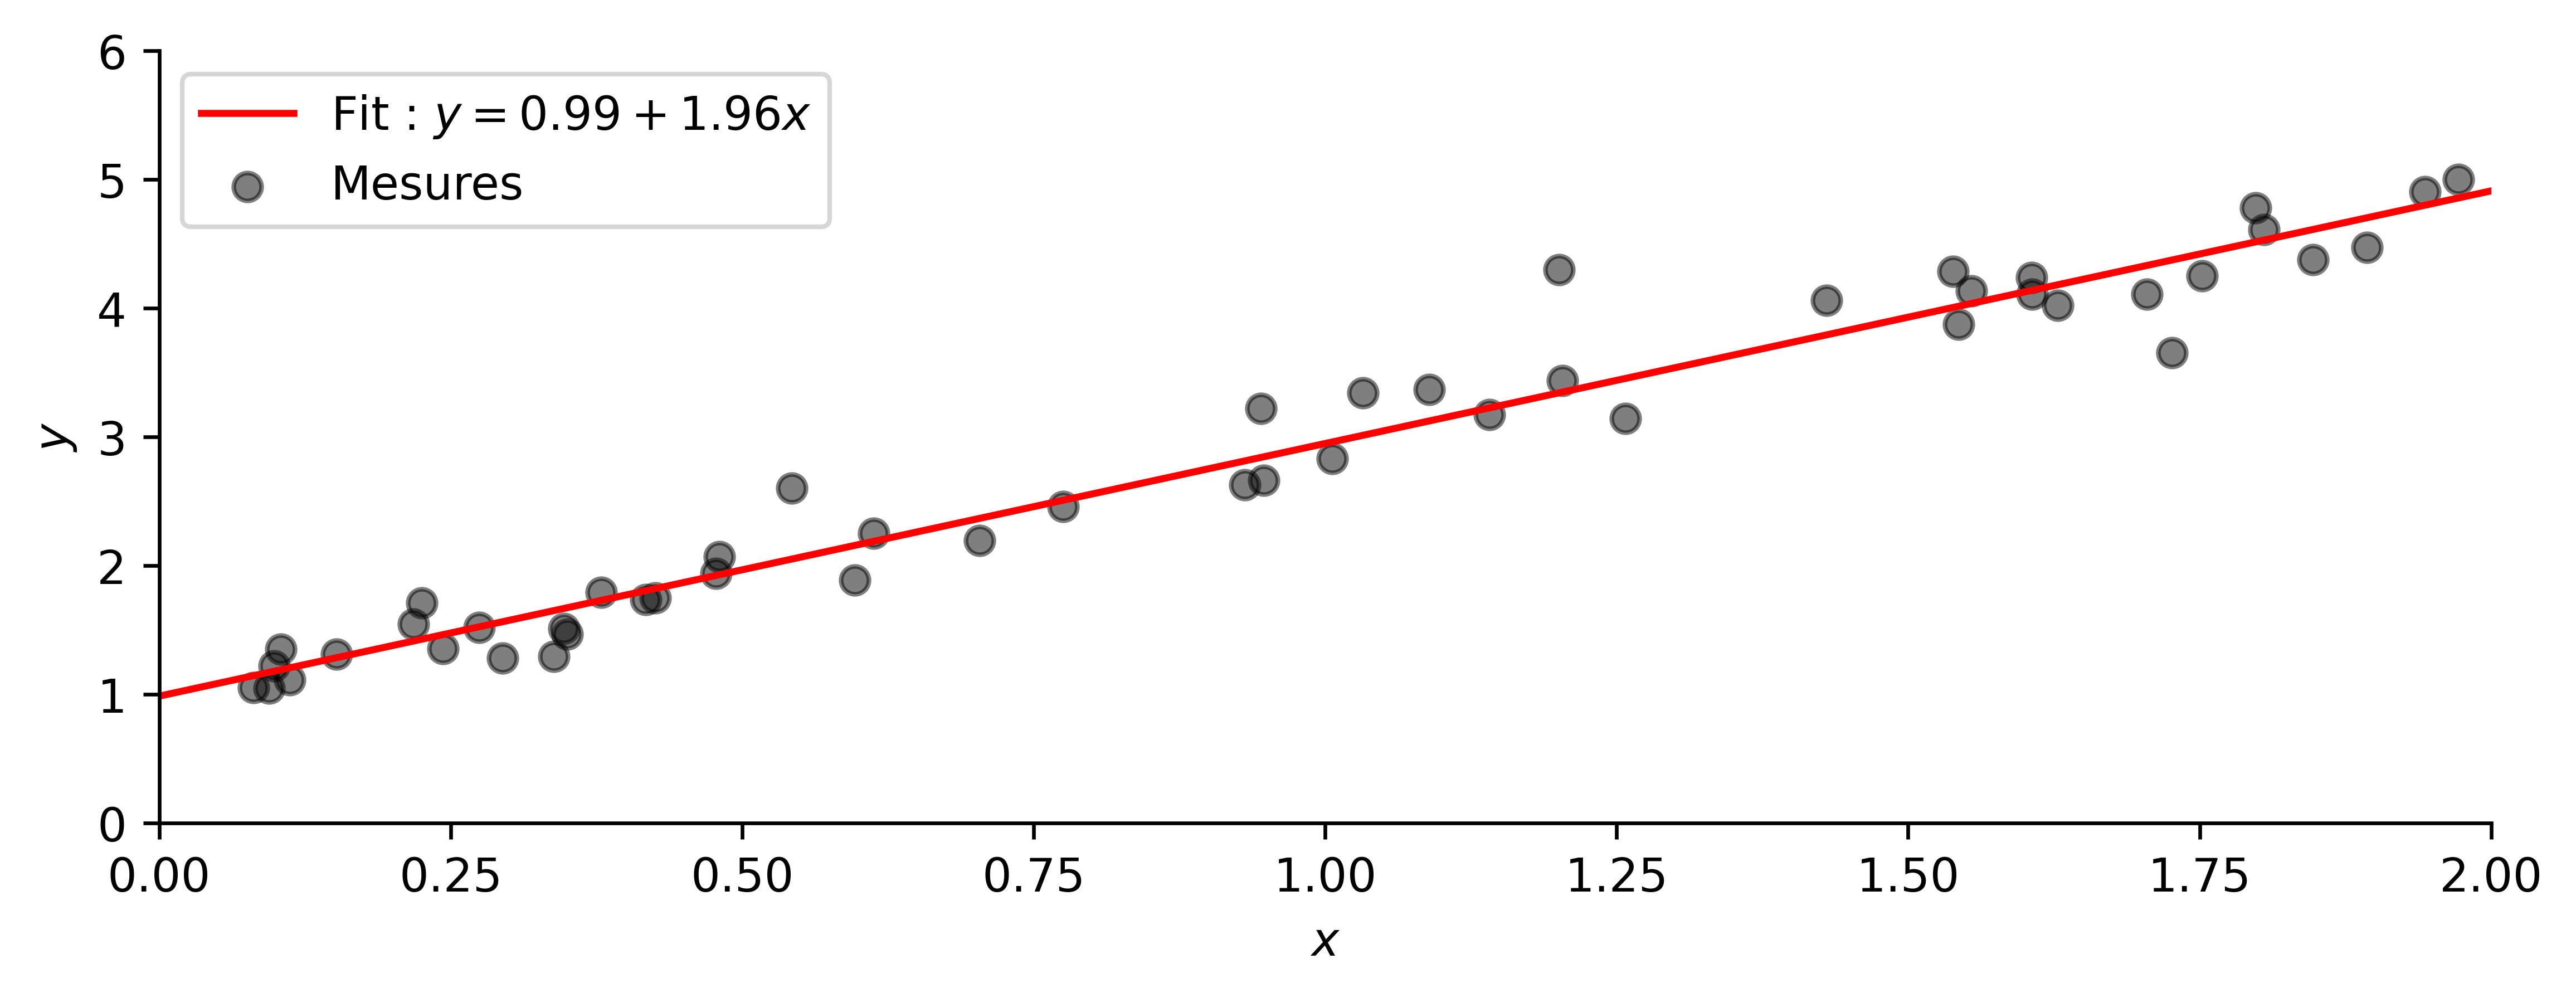
\includegraphics[width=\textwidth]{least_squares_ex}
    \vfill
  \end{frame}
}

\begin{frame}
  \centering

  
\includegraphics[width=.5\textwidth]{numpy_logo}

  Pour en savoir plus, rendez-vous sur \url{https://numpy.org/}
\end{frame}

\end{document}
